\def\QRCODE{TB_image_TUT.IMG.introduction_pythonqrcode.png}
\def\QRPAGE{http://www.iptutorials.science/tree/master/TB_image/TUT.IMG.introduction/python}
\pcorrectionsection{Python correction}

\begin{python}
# display images
import matplotlib.pyplot as plt
# ndimage defines a few filters
from scipy import misc, ndimage
# numeric calculation
import numpy as np
# measure time
import time
# read and save images
import imageio
# convolution method
from scipy.signal import convolve2d
\end{python}

\vspace*{-10pt}
\subsection{First manipulations}

\subsubsection{Open, write images}
The following file loads the ascent image and display it. The \minline{print} function is optional.

\index{Image!Load}

\begin{python}
# load file ascent
ascent = misc.ascent()
# load file cerveau.jpg
brain = imageio.imread('cerveau.jpg')
print(type(brain))
print(brain.shape, brain.dtype)
# save file
imageio.imwrite('test.png', brain)
\end{python}


\subsubsection{Display images}\index{Image!Display}
You can modify to previous example to add the following lines:
\begin{python}
plt.imshow(ascent)
plt.show()
\end{python}
Notice that you have to close the image window to write commands again. Also, the colormap is not the good one by default (see Fig. \ref{fig:introduction:python:display}).

\begin{python}
plt.figure(figsize=(10, 3.6))
# first subplot
plt.subplot(131)
plt.imshow(ascent)
# second subplot
plt.subplot(132)
plt.imshow(ascent, cmap=plt.cm.gray)
plt.axis('off')
# third subplot (zoom)
plt.subplot(133)
plt.imshow(ascent[200:220, 200:220], cmap=plt.cm.gray, interpolation='nearest')
plt.subplots_adjust(wspace=0, hspace=0., 
                    top=0.99, bottom=0.01, 
                    left=0.05, right=0.99)
plt.show()
\end{python}

\begin{figure}[H]
\centering\caption{Displaying images with an adapted colormap.}%
 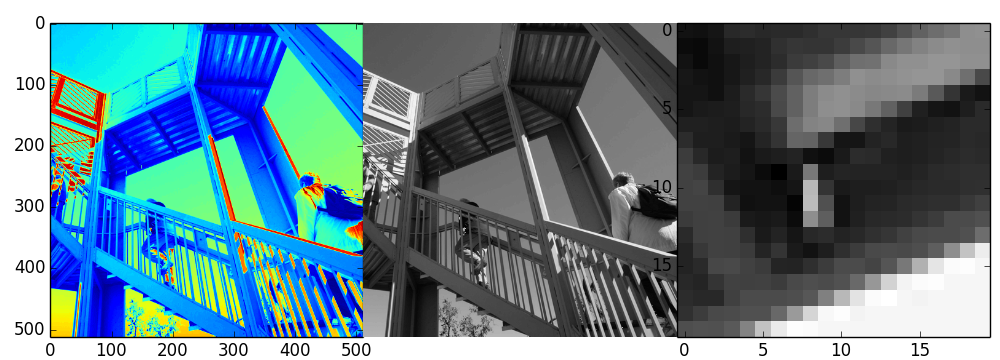
\includegraphics[height=4cm]{subplots.png}%
 \label{fig:introduction:python:display}%
\end{figure}

\subsubsection{Color channels}
A color image is constituted of (generally) three channels. This representation follows the human visual perception principles: in the human retina, the sensitive cells (the cones) react to specific wavelength that correspond to red, green and blue. The sensors technology adopted the \textit{same} characteristics and a so-called Bayer filter has 2 green filters for 1 red and 1 blue. Consequently, the green channel presents a better resolution than the other channels.

\begin{figure}[H]
 \centering\caption{The green channel presents the best contrasts in the case of retina images.}%
 \subfloat[Color image.]{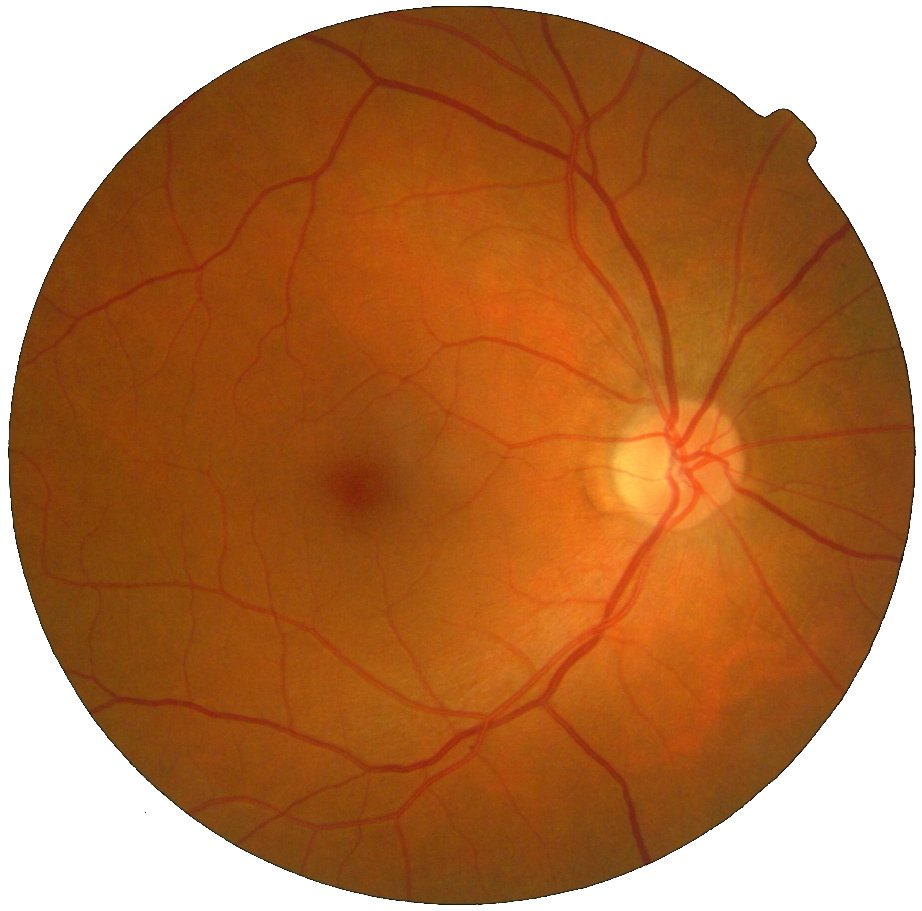
\includegraphics[width=.24\linewidth]{retine.png}}\hfill
 \subfloat[Red channel.]{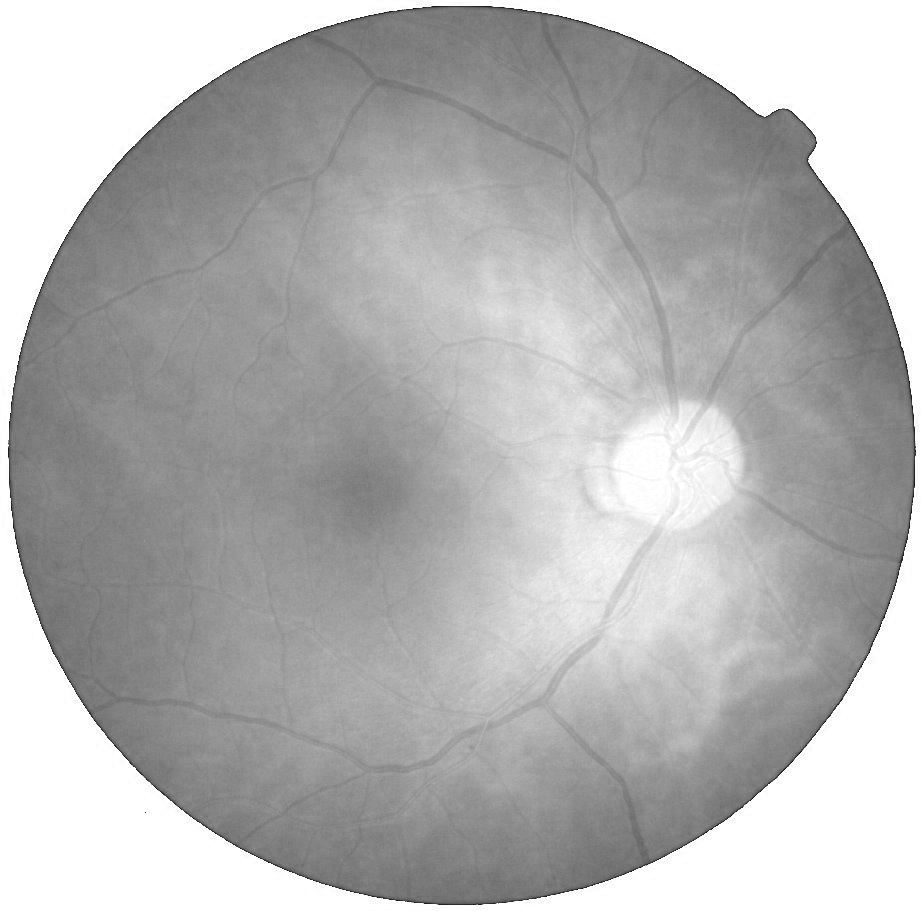
\includegraphics[width=.24\linewidth]{retine_0.python.png}}\hfill
 \subfloat[Green channel]{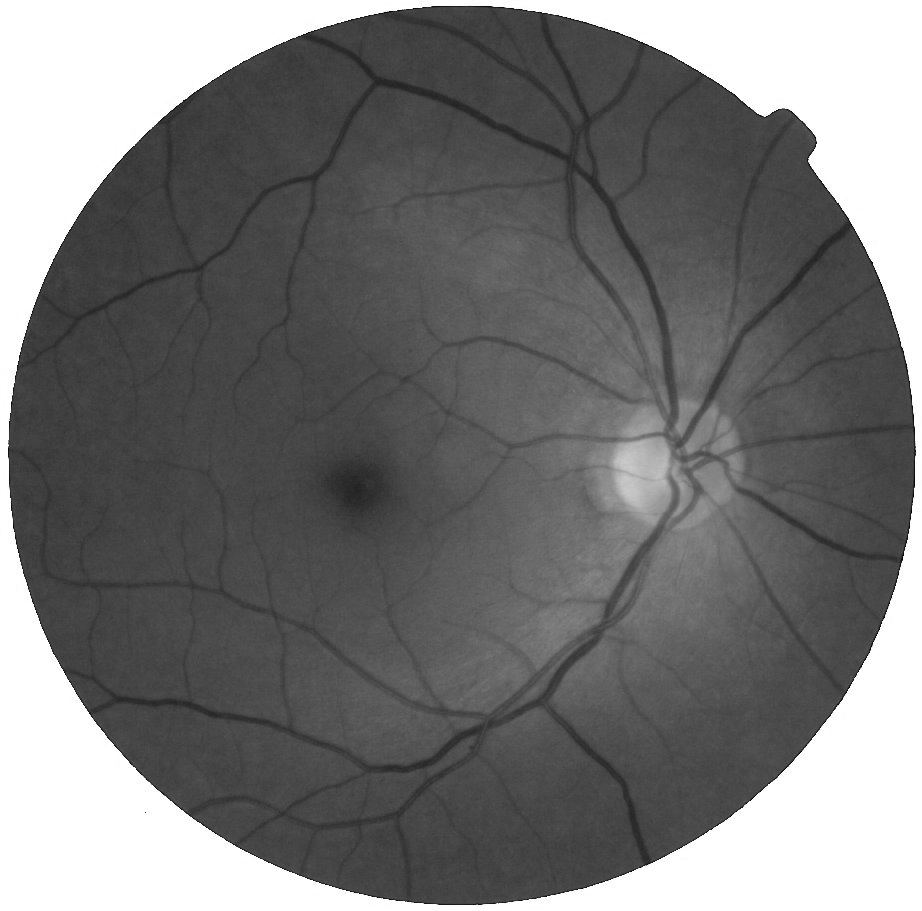
\includegraphics[width=.24\linewidth]{retine_1.python.png}}\hfill
 \subfloat[Blue channel.]{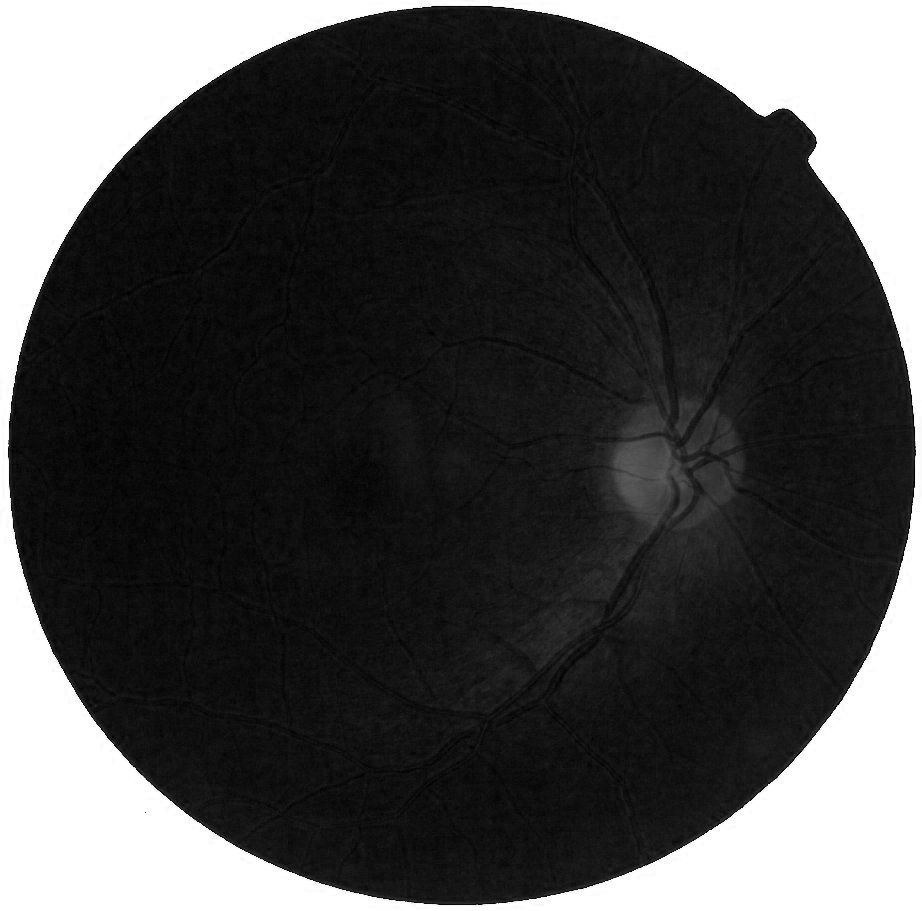
\includegraphics[width=.24\linewidth]{retine_2.python.png}}%
 \label{fig:introduction:python:channels}%
 \vspace*{-10pt}%
\end{figure}


\subsubsection{Image Resizing}\index{Resizing}
The number of pixels is reduced by subsampling the image. Notice that there is no anti-aliasing filter applied to the image before reducing its size. The result is presented in Fig.\ref{fig:introduction:python:resizing} with images of the same size, and in Fig.\ref{fig:introduction:python:resolution} with images at the same resolution.

\begin{figure}[H]
 \centering\caption{Reduction of the scale of the image on each axis, showing a so-called \textit{pixellisation} effect. Represented at the same size, the density of pixels is thus reduced.}%
 \subfloat[Scale divided by 20.]{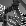
\includegraphics[width=.28\linewidth]{r20.python.png}}\hfill
 \subfloat[Scale divided by 10.]{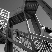
\includegraphics[width=.28\linewidth]{r10.python.png}}\hfill
 \subfloat[Scale divided by 5.]{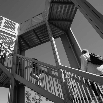
\includegraphics[width=.28\linewidth]{r5.python.png}} %\hfill
 %\subfloat[Scale divided by 2.]{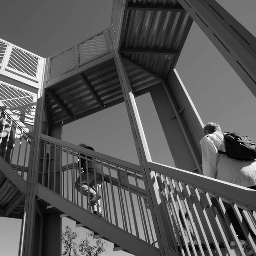
\includegraphics[width=.45\linewidth]{r2.python.png}}
 \label{fig:introduction:python:resizing}
\end{figure}

\vspace*{-7mm}

\begin{figure}[H]
 \centering\caption{At a constant resolution, images with different definitions are represented with different sizes.}%
 \subfloat[]{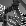
\includegraphics[width=.07\linewidth]{r20.python.png}}\hspace{1cm}
 \subfloat[]{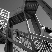
\includegraphics[width=.14\linewidth]{r10.python.png}}\hspace{1cm}
 \subfloat[]{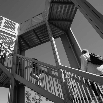
\includegraphics[width=.28\linewidth]{r5.python.png}} %\hfill
 %\subfloat[Scale divided by 2.]{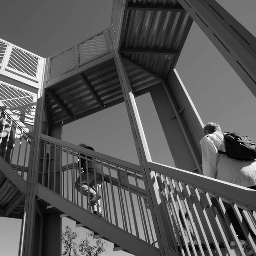
\includegraphics[width=.45\linewidth]{r2.python.png}}
 \label{fig:introduction:python:resolution}%
\end{figure}


\subsubsection{Color quantization}\index{Quantization}
The following code uses the properties of integer operations to round values to the nearest integer. Illustration is presented Fig. \ref{fig:introduction:python:quantization}.

\begin{python}
q4 = ascent // 4*4;
q16= ascent //16*16;
q32= ascent //32*32;
\end{python}

\vspace*{-3mm}

\begin{figure}[H]
 \centering\caption{Reduction of the number of gray levels (quantization).}
 \subfloat[q4.]{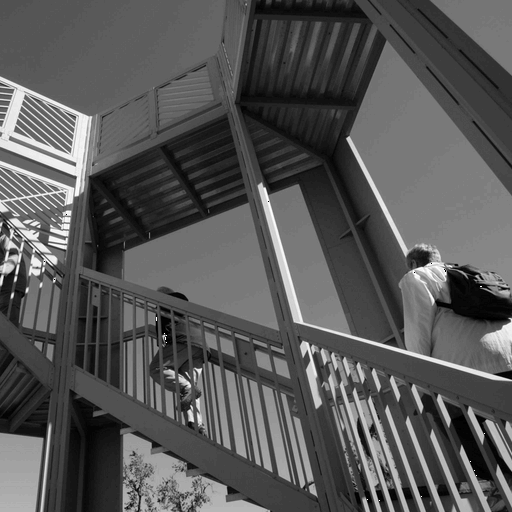
\includegraphics[width=.28\linewidth]{q4.python.png}}\hfill
 \subfloat[q16.]{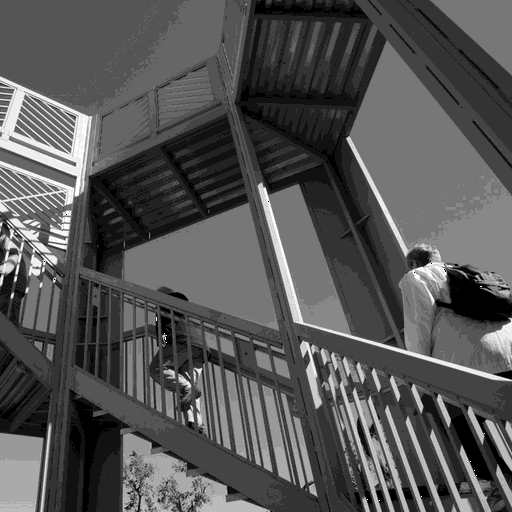
\includegraphics[width=.28\linewidth]{q16.python.png}}\hfill
 \subfloat[q32.]{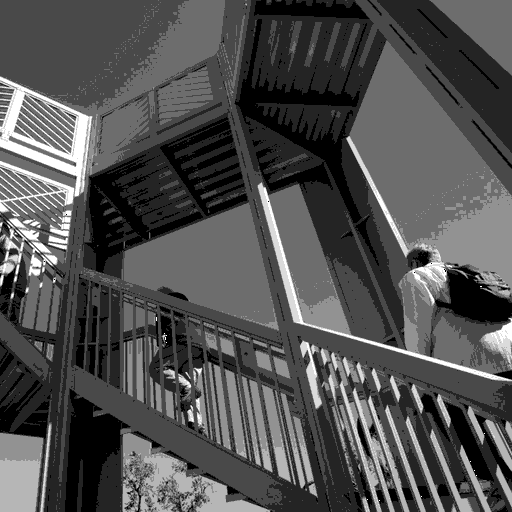
\includegraphics[width=.28\linewidth]{q32.python.png}}%
 \label{fig:introduction:python:quantization}%

\end{figure}


\subsubsection{JPEG file format}
In order to test the effect of jpeg compression, one can use the parameter \pinline{quality}. For the lowest quality, the loss of informations is really important (see Fig.\ref{fig:introduction:python:jpeg}).
\begin{python}
# test jpeg quality
imageio.imwrite("a_25.python.jpeg", ascent, quality=25);
imageio.imwrite("a_100.python.jpeg", ascent, quality=100);
imageio.imwrite("a_50.python.jpeg", ascent, quality=50);
imageio.imwrite("a_75.python.jpeg", ascent, quality=75);
imageio.imwrite("a_1.python.jpeg", ascent, quality=1);
\end{python}

\begin{figure}[H]
 \centering\caption{Different quality used to compress jpeg files.}%
 \subfloat[Quality 1.]{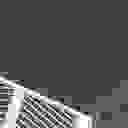
\includegraphics[width=.28\linewidth]{a_1.python.jpeg}}\hfill
 \subfloat[Quality 25.]{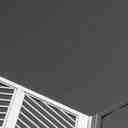
\includegraphics[width=.28\linewidth]{a_25.python.jpeg}}\hfill 
 \subfloat[Quality 75.]{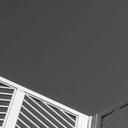
\includegraphics[width=.28\linewidth]{a_75.python.jpeg}}%
 \label{fig:introduction:python:jpeg}%
\end{figure}



\subsection{Histogram}\index{Histogram}
To plot the histogram of an image, you can use the hist function (see result in Fig. \ref{fig:histo}).
\begin{python}
plt.hist(ascent.flatten(), 256)
plt.show()
\end{python}
\begin{figure}[H]
 \centering\caption{Histogram of ascent image.}%
 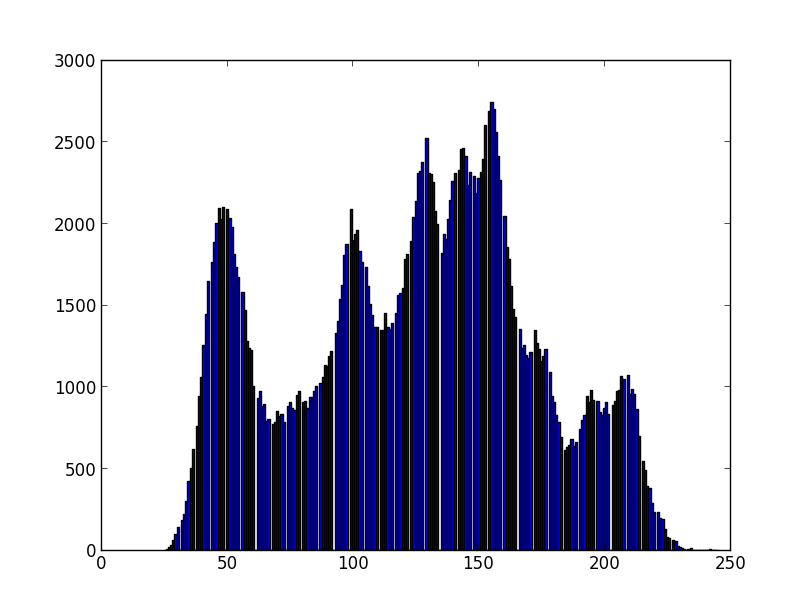
\includegraphics[width=8cm]{histo.png}%
 \vspace*{-5pt}%
 \label{fig:histo}%
\end{figure}

You can also write your own code. The execution time is higher for these two functions than for the previous one.
\begin{python}
# Histogram function with 2D image
def compute_histogram(image):
    tab = np.zeros((256, ), dtype='I')
    X, Y = image.shape
    for i in range(X):
        for j in range(Y):
            tab[image[i,j]]+=1

    return tab
\end{python}
    
\begin{python}
# Histogram function with flatten image (vector)
def compute_histogram2(image):
    im = image.flatten() 
    tab = np.zeros((256, ), dtype='I')
    for i in im:
        tab[i]+=1
    return tab
\end{python}

The following code presents a comparison of the different method for histogram computation.

\begin{python}
# load ascent image and compute histograms
ascent = misc.ascent()
t0 = time.clock()
h = compute_histogram(ascent)
t1 = time.clock()
h2=compute_histogram2(ascent)
t2 = time.clock()
# .... plots
print "execution time 2D:%g" %(t1-t0)
plt.subplot(131)
plt.plot(h)
plt.title('2D function')

print "execution time 1D:%g" %(t2-t1)
plt.subplot(132)
plt.plot(h2)
plt.title('1D function')
# last plot: with matplotlib function
plt.subplot(133)
t3 = time.clock()
plt.hist(ascent.flatten(), 256)
t4 = time.clock()
print "execution time matplotlib:%g" %(t4-t3)
# display
plt.show()
\end{python}
The console outputs the following computation durations:
\begin{sh}
execution time 2D: 1.40284 s
execution time 1D: 1.27649 s
execution time matplotlib: 0.261095 s
\end{sh}


\subsection{Linear mapping of the image intensities}\index{Mapping}
The linear mapping is a simple method that stretches linearly the histogram. If displayed with \pinline{matplotlib}, the images is linearly stretched, thus the modification cannot be observed.

\begin{python}
def image_stretch(image):
	# return image with new maximum and minimum at 255 and 0
	minimum = image.min();
	maximum = image.max();
	a = 255/(maximum-minimum);
	b = -255*minimum/(maximum-minimum);
	return a*image+b;
\end{python}


\subsection{Aliasing effect}\index{Aliasing}
\begin{python}
# aliasing effect (Moire)
def circle(fs, f):
    # Generates an image with aliasing effect
    # fs: sample frequency
    # f : signal frequency
    t = np.arange(0,1,1./fs);
    ti,tj = np.meshgrid(t,t);
    C = np.sin(2*np.pi*f*np.sqrt(ti**2+tj**2));
    return C
\end{python}

The image of Fig. \ref{fig:introduction:python:aliasing} is generated with the following code.

\begin{python}
C = circle(300,50);
plt.imshow(C, cmap=plt.cm.gray);
plt.show()
imageio.imwrite('moire.png', C);
\end{python}

\begin{figure}[H]
 \centering\caption{Moiré effect, generated with $f_s=300$ and $f=50$.}%
 \vspace*{-2pt}%
 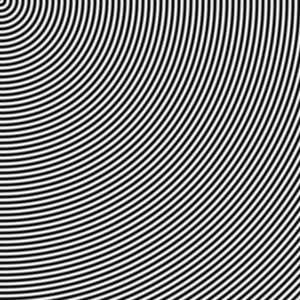
\includegraphics[width=8.5cm]{moire.png}%
 \vspace*{-10pt}%
 \label{fig:introduction:python:aliasing}%
\end{figure}


\subsection{Low-pass filtering}
\index{Filtering!Low-pass}
\begin{pcomment}
\begin{premark}The module \minline{scipy.ndimage.filters} contains the usual filter functions. 
\end{premark}
\end{pcomment}
The mean filter is illustrated in Fig. \ref{fig:introduction:python:mean}.

\begin{python}
# mean on a 3x3 neighborhood
m3 = ndimage.filters.uniform_filter(ascent)
m25= ndimage.filters.uniform_filter(ascent, 25)

plt.subplot(121)
plt.imshow(m3, cmap=plt.cm.gray)
plt.axis('off')
plt.title('3x3 mean filter')

plt.subplot(122)
plt.imshow(m25, cmap=plt.cm.gray)
plt.axis('off')
plt.title('25x25 mean filter')

plt.show()
\end{python}

\begin{figure}[H]
 \centering\caption{Mean filters.}
 \subfloat[Neighborhood of size 3x3.]{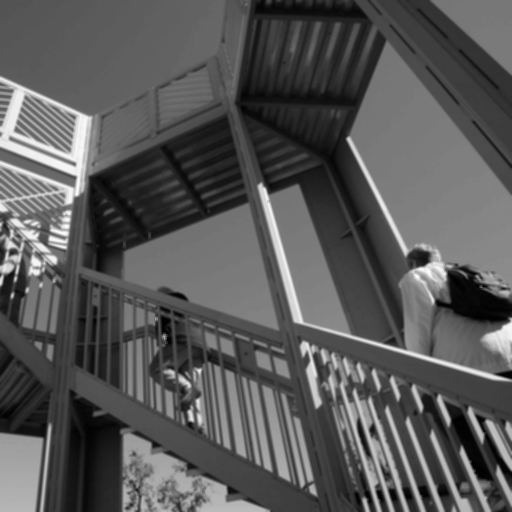
\includegraphics[height=5cm]{ascent_mean_3.png}}\hspace{1cm}
 \subfloat[Neighborhood of size 25x25.]{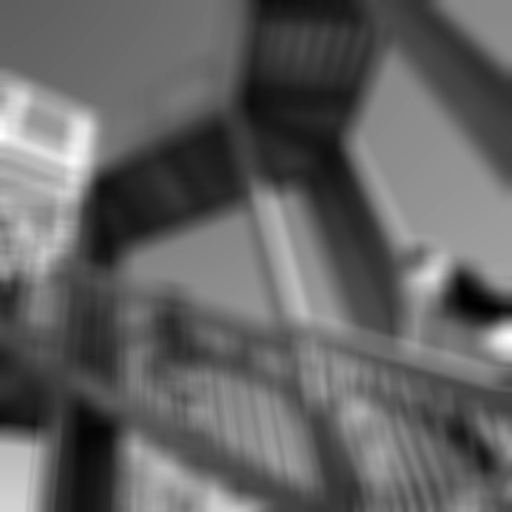
\includegraphics[height=5cm]{ascent_mean_25.png}}%
 \label{fig:introduction:python:mean}%
\end{figure}

\subsubsection{Gaussian filter}
The gaussian filter is presented in Fig. \ref{fig:introduction:python:gaussian}.
\begin{python}
# ascent image
ascent = misc.ascent()

# Gaussian filter
gaussian = ndimage.filters.gaussian_filter(ascent, 5)
\end{python}

\vspace*{-4pt}

\begin{figure}[H]
 \centering\caption{Gaussian filter of size 5.}%
 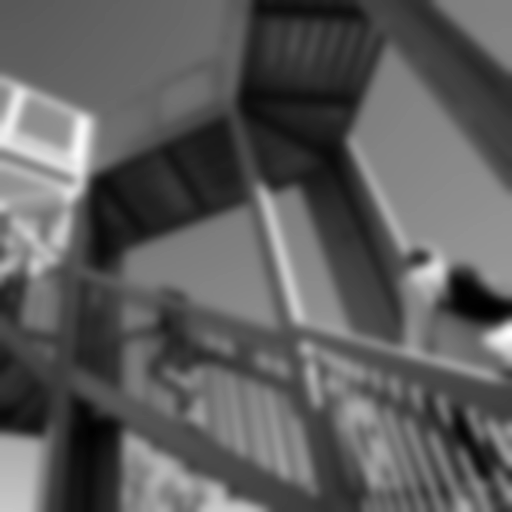
\includegraphics[width=5cm]{gaussian.png}%
 \label{fig:introduction:python:gaussian}%
\end{figure}

\subsection{High-pass filter}
The computation of the high-pass filter is simply the subtraction of a low-pass filter from the original image. For example:

\begin{python}
H = I-m25
\end{python}


\vspace*{-7pt}
\subsection{Derivative filters}
\index{Filtering!High-pass}
\index{Laplacian}
\index{Gradient!Prewitt}
\index{Gradient!Sobel}
Derivative filters (Prewitt, Sobel...) use a finite derivation approximation. They are very sensitive to noise (as every system using a derivation). The gradient is defined as a vector, and a norm should be used to display a resulting image. Notice that with these filters, the connexity of the contours is not preserved.
Illustration is proposed in Fig. \ref{fig:introduction:python:prewitt}.

\begin{python}
# ascent image
ascent = misc.ascent()
ascent.astype('int32');

# Prewitt filter
prewitt0 = ndimage.filters.prewitt(ascent, axis=0)
prewitt1 = ndimage.filters.prewitt(ascent, axis=1)

# Sobel filter
dy = ndimage.filters.sobel(ascent, axis=0) # vertical
dx = ndimage.filters.sobel(ascent, axis=1) # horizontal
mag = np.hypot(dx, dy)  # magnitude
sobel = mag * 255.0 / mag.max()  # normalize (Q&D)

# display results
plt.subplot(131)
plt.imshow(prewitt0, cmap=plt.cm.gray)
plt.axis('off')
plt.title('Prewitt filter axis 0')

plt.subplot(132)
plt.imshow(prewitt1, cmap=plt.cm.gray)
plt.axis('off')
plt.title('Prewitt filter axis 1')

plt.subplot(133)
plt.imshow(sobel, cmap=plt.cm.gray)
plt.axis('off')
plt.title('Sobel filter')

plt.show()
\end{python}

\begin{figure}[H]
\centering\caption{Prewitt filter.}
\subfloat[Prewitt filter for axis x.]{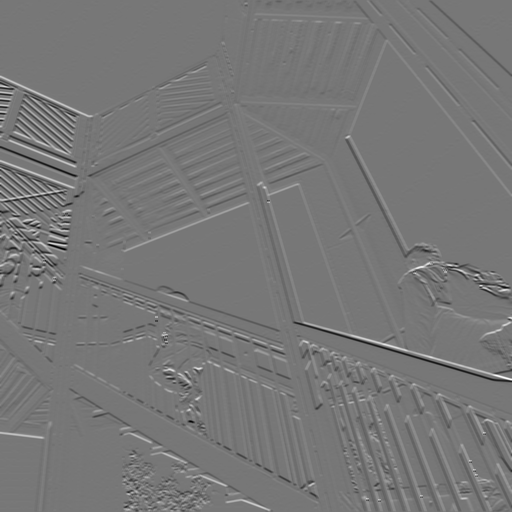
\includegraphics[width=5cm]{prewitt0.png}}\hspace{1.5cm}
\subfloat[Prewitt filter for axis y.]{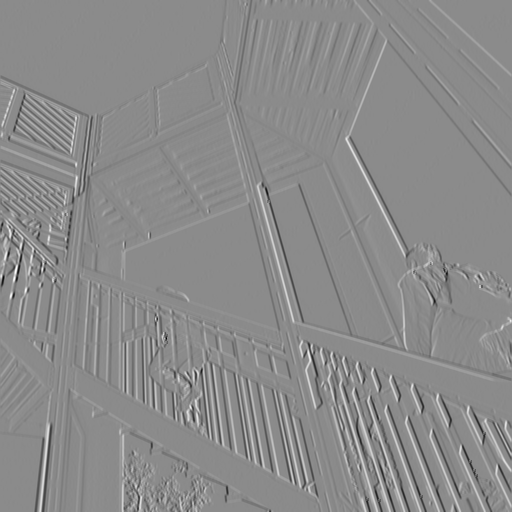
\includegraphics[width=5cm]{prewitt1.png}}
\label{fig:introduction:python:prewitt}
\end{figure}

The previous code uses filters proposed by the \pinline{skimage} module. If you want to write down the convolution matrix, this is the solution:
\begin{python}
h = np.array([[-1, 0, 1], [-1, 0, 1], [-1, 0, 1] ])
grad1 = convolve2d(ascent, h);
plt.imshow(grad1, cmap=plt.cm.gray)
plt.show()

grad0 = convolve2d(ascent, h.transpose());
plt.imshow(grad0, cmap=plt.cm.gray)
plt.show()

plt.imshow(np.sqrt(grad0**2 + grad1**2), cmap=plt.cm.gray)
plt.show()
\end{python}


\subsection{Enhancement filter}

This functions adds the Laplacian filter to the original image.
\begin{python}
def sharpen(I, alpha):
    
    h = np.array([[-1, -1, -1], [-1, 8, -1], [-1, -1, -1] ])
    L = convolve2d(I, h, mode='same')
    np.max(L)
    E = alpha * I + L
    E = skimage.exposure.rescale_intensity(E, out_range=(0,255))
    E = E.astype(np.uint8)
    
    return E
\end{python}

This constitutes a really simple and efficient edge sharpening method. To test it, you may write this example code:
\begin{python}
I = skimage.io.imread('osteoblaste.png').astype(np.float)
I = I/255
A = [1, 0.5, 5]

fig = plt.figure(figsize=(12,8))
plt.subplot(221)
plt.imshow(I, cmap=plt.cm.gray)
for i,alpha in enumerate(A):
    plt.subplot(222+i)
    E = sharpen(I, alpha)
    E = skimage.exposure.rescale_intensity(E, out_range=(0,255))
    plt.imshow(E, cmap=plt.cm.gray)
    plt.title('alpha='+str(alpha))
    
    skimage.io.imsave('osteoblaste_rehauss_'+str(alpha)+'.python.png', E)

plt.show()
\end{python}


\begin{figure}[htbp]
 \centering
 
 \subfloat[$\alpha=1$.]{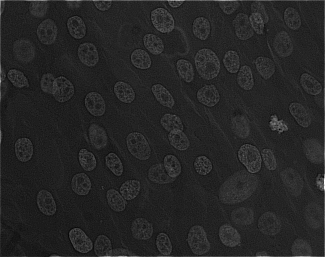
\includegraphics[width=5cm]{osteoblaste_rehauss_1.python.png}}
 \hspace{1cm}
 \subfloat[$\alpha=0.5$.]{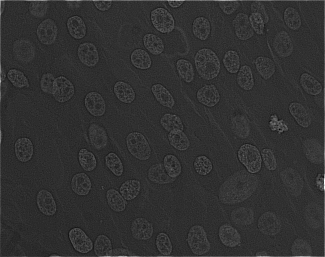
\includegraphics[width=5cm]{osteoblaste_rehauss_0.5.python.png}}
 
 \subfloat[$\alpha=5$.]{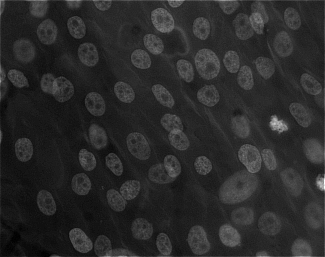
\includegraphics[width=5cm]{osteoblaste_rehauss_5.python.png}}
 \hspace{1cm}
 \subfloat[Original image.]{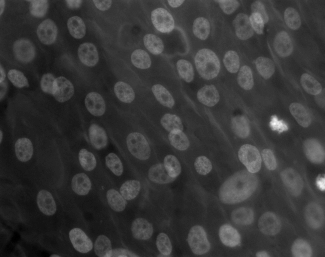
\includegraphics[width=5cm]{osteoblaste.png}}

 \caption{Image enhancement: $I=\alpha\cdot I+HP(I)$, where $HP$ is a high-pass filter (the Laplacian filter in these illustrations).}
 \label{fig:introduction:matlab:enhancement}
\end{figure}
